\documentclass{article}

\usepackage{listings}
\usepackage{graphicx}
\usepackage{color}

\lstset{numbersep=5pt,numbers=left,numberstyle=\footnotesize,title=\lstname,basicstyle=\footnotesize,showspaces=false,breaklines=true}

\begin{document}

\title{Knapsack problem - Dynamic programming}

\author{Jander Nascimento}

\maketitle

\tableofcontents

\section{Recursive algorithm}

Here,is the recursive algorithm\cite{algojava} that can be used to obtain the optimal value of the knapsack.

\begin{lstlisting}
//Max function that returns the biggest value among the two parameters passed.
recDP(int[] w,int[] p, int i, int j){
  if i=0 OR j=0 then 
    return 0;
  fi

  if w[i-1]>j then
    return recDP(w,p,i-1,j)
  fi

  if w[i-1]<=j then
    return Max(recDP(w,p,i-1,j),
 		p[i-1]+recDP(w,p,i-1,j-w[i-1])
  fi
}
\end{lstlisting}

The running cost of the algorithm is proportional to the number of itens. Mathematically, let's consider
the function T(n) the function that express the running time. Using the function before we may define as 
T(n)=nW and space used is the same O(nW).

The formulation of the problem is:

\[
  A(i,j) = \left\{ 
  \begin{array}{l l}
    0 & \quad \textnormal{if $i$ = 0 or $j$ = 0}\\
    A(i-1,j) & \quad \textnormal{if $w_i$ \textgreater j}\\
    max\{A(i-1,j),v_i+A(i-1,j-w_i)\} & \quad \textnormal{if $w_i$ \textless= j}\\
  \end{array} \right.
\]



\section{Sequencial algorithm}          

\begin{lstlisting}
//Max function that returns the biggest value among the two parameters passed.
//w array with weights
//p array with prices
//W knapsack maximum weight
//n total number of itens
seqDP(int w[],int p[],int W,int n){

  for i:=0 to W do
    knap[0][i]:=0
  od

  for k:=1 to n do
    knap[k][0]:=0
    for y:=1 to W do
      if y < w[k-1] then
        knap[k][y]:=knap[k-1][y]
      else
        knap[k][y]:=Max(knap[k-1][y],
			p[k-1]+knap[k-1][y-w[k-1]])
      fi

  return knap[n][W]

}
\end{lstlisting}


\section{Is Recovering the reason for optmal solution?}          

\section{SeqDP and RecDP \textit{versus} Brute-force and Greedy}

\subsection{Time analysis}

Here is a chart which displays the behaviour of our algorithm according to time.

\begin{figure}
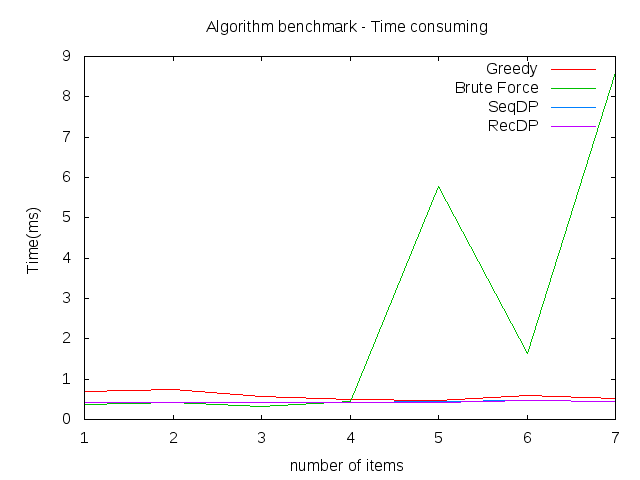
\includegraphics[scale=0.4]{report/time_analysis}
\caption{Algorithms comparison: timing}
\label{report/time_analysis}
\end{figure}

\subsection{Price analysis}

As the time is our only contraint we are evaluating an algorithm, we used the price of the knapsack
as a variable to be analyzed. Since this variable denotates how efficience our algorithm was, in terms 
of price.

\begin{figure}
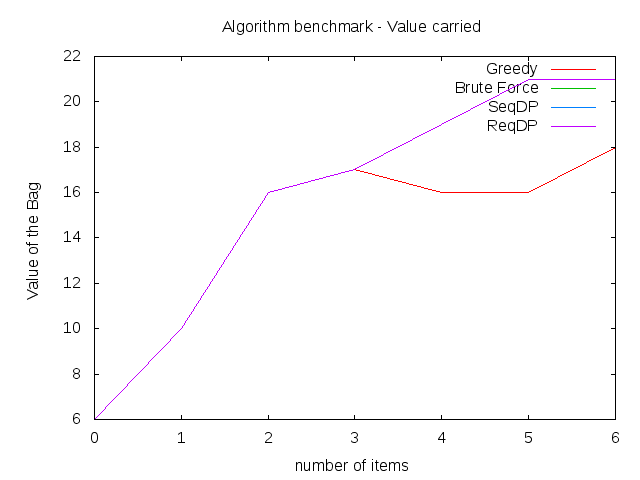
\includegraphics[scale=0.4]{report/price_analysis}
\caption{Algorithms comparison: price}
\label{report/price_analysis}
\end{figure}

\subsection{What can i do with 30 sec}

As suggested, to use our best implementation, it is adopted the seqDP. It is possible to find best solution for 50000 itens 
using seqDP within 30 seconds.

\section{RecDP and array usage}

A test performed with an instance of 10 itens and knapsack maximum weight of 64 shows that the total array size created was
640 and only 220 position were indeed used, this represents only 35\% of the array.

\section{Better cases for RecDP}
	
\begin{thebibliography}{9}

\bibitem{algojava}
  Robert Sedgewick,
  \emph{Algorithms in Java}.
  Addison-Wesley, 2002,
  3rd Edition,
  1994.

\end{thebibliography}

\end{document}
